% Sample Dissertation, Thesis, or Document %
%            for use with the              %
%  University of Arizona Thesis Class,     %
%               uathesis.cls               %
%------------------------------------------%

% We'll use the uathesis document class (duh).  The uncommented line below will produce a Dissertation, the others would produce a Thesis.
% There are other options available to you like turning on the copyright statement and replacing the year on the title page with a "generated on" stamp (handy for early drafts).
% To find out what the available options are, take a look into the uathesis.cls file and look for the commands near the top of that file.
% There are five copyright options.  Copyright, no copyright, and three different Creative Commons licenses.
% The draft and Final options are also recommended.  The draft option will enable faster compile time and the final option will turn off todo notes.

%\documentclass[dissertation]{uathesis}
%\documentclass[dissertation,copyright]{uathesis}
%\documentclass[dissertation,CC-BY]{uathesis}
%\documentclass[dissertation,CC-BY-SA]{uathesis}
\documentclass[dissertation,CC-BY-ND,generatedon]{uathesis}
%\documentclass[dissertation,generatedon]{uathesis}
%\documentclass[thesis]{uathesis}
%\documentclass[document]{uathesis}

%% These are other packages that you might find useful.

%\usepackage{callouts} % for callouts in the document
%\usepackage{todonotes} % for todo notes while writing the document, turn off with final option
%\usepackage{siunitx} % Comprehensive package for typesetting units
\usepackage{lipsum} % For dummy text

%% Use biblatex for bibliography management. Set here for different styles if required. Default is IEEE
\usepackage[style=ieee]{biblatex}
\DefineBibliographyStrings{english}{% Redifine bibliography tile name
  bibliography = {REFERENCES},
  references = {REFERENCES},
}

%% Add your bibliography file(s) here.
\addbibresource{bibliography.bib}

%% hyper-ref typically has to go last in the list of packages, force newer pdf version for embedding approval.
\usepackage[bookmarks,colorlinks=true,urlcolor=red,linkcolor=black,citecolor=black,xetex,pdfversion=1.7]{hyperref} 
\usepackage{cleveref} % for smart cross-reference, must be enabled after hyperref

%% Pdf metadata
\hypersetup{%
  pdftitle={Your PDF title},
  pdfsubject={Your PDF subject},
  pdfauthor={Your PDF author},
  pdfkeywords={Your PDF keywords},
}

%% Toggle to only render selected chapters, comment out to skip chapter, references and labels will still work. remember to add all input files.
\includeonly{%
  introduction.tex,
  previous_work.tex,
  appendix-A.tex}

\begin{document}
\frontmatter* % Chapters here don't count and input is used instead of include
%% Set up the title page
% \maketitlepage{Title}{Author}{degree title}{Department}{year}
\maketitlepage%
{My Lovely Dissertation} % Title of your Thesis/
{Wilber WildCat} % Grad college wants your full name here.
{Doctor of Philosophy} % Title of your degree.
{WYANT COLLEGE OF OPTICAL SCIENCE} % Title of your department.
{2023} % Year of degree

%% Insert the approval form, no need to print since electronic workflow is preferred.
%  See ua-template directory for more samples and instructions.
%  Will automatically add page numbers to the approval form.
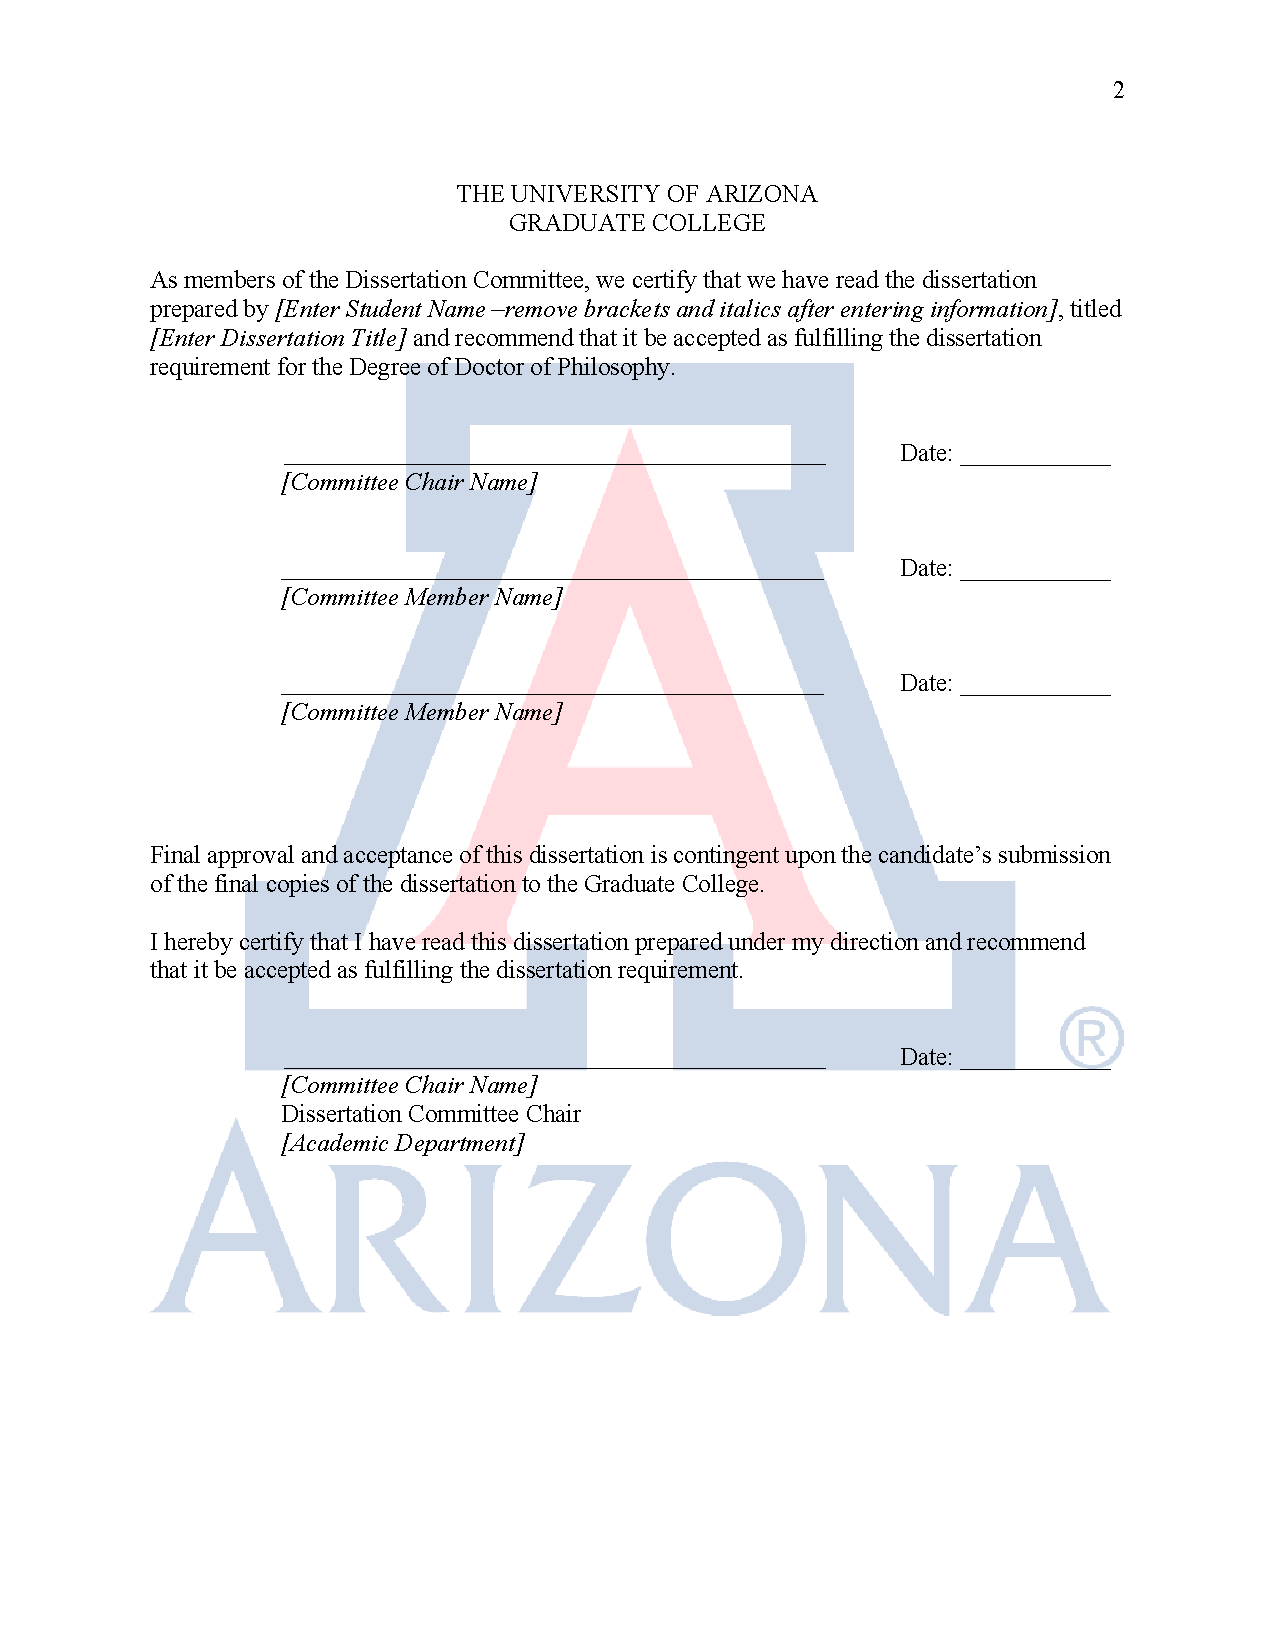
\includepdf[pagecommand={}]{approval-sample.pdf}

% Include the OPTIONAL``Acknowledgements''
\chapter{Acknowledgements}
Thanks to all the previous students that contributed to this project.

\begin{itemize}
    \item Peter Halverson	1989 (non-LPL)
    \item William D. Sears	1994 (Department of Planetary Sciences)
    \item Rov Vervack		1996 (Department of Planetary Sciences)
    \item Andrew Rivkin	1997 (Department of Planetary Sciences)
    \item Joe Spitale		2001 (Department of Planetary Sciences)
    \item Dave O'Brien		2003 (Department of Planetary Sciences)
    \item Ross A. Beyer	2004 (Department of Planetary Sciences)
    \item Jim Richardson	2005 (Department of Planetary Sciences)
    \item Terry Hurford	2005 (Department of Planetary Sciences)
    \item Curtis S. Cooper	2007 (Department of Planetary Sciences)
    \item David A. Minton  2009 (Department of Planetary Sciences)
    \item Anh X. Tran		2013 (Department of Computer Sciences)
    \item Ted Lee		2023 (Wyant College of Optical Sciences)
\end{itemize}

This would not have been possible without the past work and foundation laid by the previous students.

\chapter{Land ACKNOWLEDGEMENT}
We respectfully acknowledge the University of Arizona is on the land and territories of Indigenous peoples.
Today, Arizona is home to 22 federally recognized tribes, with Tucson being home to the O'odham and the Yaqui.
Committed to diversity and inclusion, the University strives to build sustainable relationships with sovereign Native Nations and Indigenous communities through education offerings, partnerships, and community service.


% Include the OPTIONAL ``Dedication''
\chapter{Dedication}
\begin{center}
\emph{Dedicated to some nice folks.}
\end{center}



% Create a ``Table of Contents''
\tableofcontents
\cleardoublepage
% Create a ``List of Figures''
\listoffigures
\cleardoublepage
% Create a ``List of Tables''
\listoftables
\cleardoublepage

% Include the ``Abstract''
%% Abstract is typeset differently than the rest of the document, so we need to use a separate environment.
\abstractintoc %include abstract in table of contents

\begin{abstract}
    This is the abstract. It should be a short summary of the thesis.

    \lipsum[4]

\end{abstract}


\mainmatter*

% Include the various chapters, remember to add them to the \includeonly{} list above.
\chapter{INTRODUCTION\label{chapter:introduction}}

\lipsum

\section{Overview\label{sec:overview}}

\lipsum[1]

This is a sample citation \autocite{Bob2011}.
\lipsum[2]

Lets try a \cref{chapter:introduction} reference.
Now lets see how to add a Figure float.

\begin{figure}
    \centering % Center the figure
    \includegraphics{example-image-a} % Most image formats are supported
    \caption{This is a sample figure.\label{fig:samplefigure}} % Good habit to add labels in captions.
\end{figure}

After a figure, referenced as \cref{fig:samplefigure}.
Let's try a table now.
\begin{table}
    \centering
    \caption{My Sample Table\label{tab:sampletable}}
    \begin{tabular}{c c c}
        \toprule
        \multicolumn{3}{c}{Sample Table} \\
        \midrule
        Column 1 & Column 2 & Column 3 \\
        \midrule
        1 & 2 & 3 \\  
        Some text & More text & Even more text \\
        \bottomrule
    \end{tabular}
\end{table}
\chapter{PREVIOUS WORK\label{chap:previousWork}}

\lipsum

% Include the various appendices, remember to add them to the \includeonly{} list above.
\appendix

\chapter{Sample Appendix\label{apndxA}}

\lipsum



\backmatter

% Create the References list
\printbibliography

\end{document}